\section{Mikrofone}
\subsection{Richtcharakteristik}
\begin{quote}
"Die Richtcharakteristik definiert, aus welcher Richtung das Mikrofon den Schall besonders empfindlich aufnimmt. Stark vereinfacht gesagt: Aus welcher Richtung aufgenommen wird." (https://www.delamar.de/mikrofon/richtcharakteristik-mikrofon-22647/ [Zugriff: 17.03.2018])
\end{quote}
\subsubsection{Kugelcharakteristik}
Bei der Kugelcharakteristik wird der Schall von allen Richtungen aufgenommen, das heißt es wird von keiner bevorzugten Richtung aufgenommen. Das Problem, was dadurch entsteht, ist, dass die Rückkoppelanfälligkeit sehr hoch ist, wodurch Mikrofone mit einer Kugelcharakteristik schlecht für Bühnen geeignet sind.\citep{kugel}
\begin{figure}[H]
	\centering
	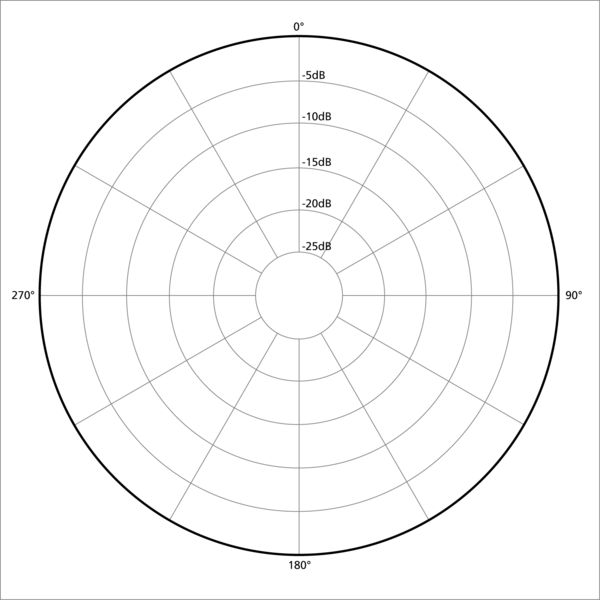
\includegraphics[width=0.4\textwidth]{abb4} 
	\caption[Kugel]{Kugel\footnotemark}
\end{figure}
\footnotetext{Quelle: https://www.delamar.de/mikrofon/richtcharakteristik-mikrofon-22647/}
\subsubsection{Nierencharakteristik}
Die Niere nimmt, im Gegensatz zur Kugelcharakteristik, aus einer bevorzugten Richtung auf. Im Gegensatz zu der Kugelcharakteristik, bei der der Schall von allen Seiten aufgenommen wird, wird er bei der Niere nur von einer Seite aufgenommen, meistens von vorne. Der Schall wird von den Seiten nur sehr leise bis gar nicht aufgenommen. Der Vorteil der Niere ist, dass sie rückkopplungsfester, als die Kugel ist und sie so auch beispielsweise bei Konzerten verwendet werden kann. Der Nachteil der Niere ist der sogenannte Nahbesprechungseffekt.\citep{naheffekt}\citep{kugel} Das bedeutet: "Ab einer gewissen Nähe der Schallquelle werden die tieffrequenten Anteile dominanter." (https://www.delamar.de/faq/nahbesprechungseffekt-34021/ [Zugriff: 17.03.2018])
\begin{figure}[H]
	\centering
	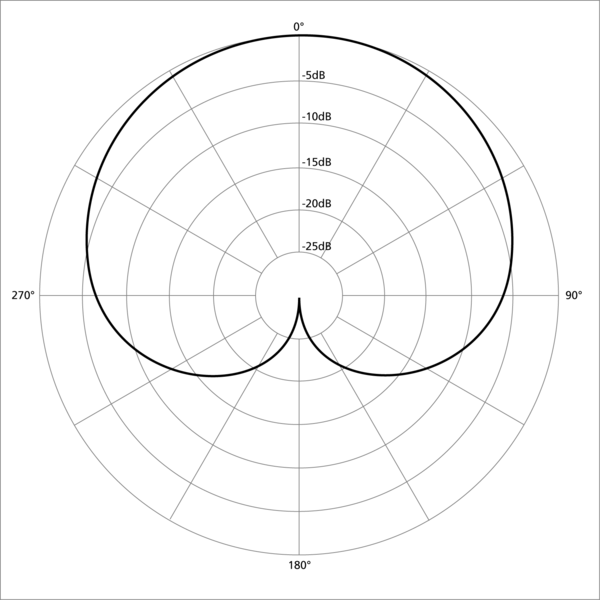
\includegraphics[width=0.4\textwidth]{abb5} 
	\caption[Niere]{Niere\footnotemark}
\end{figure}
\footnotetext{Quelle: https://www.delamar.de/mikrofon/richtcharakteristik-mikrofon-22647/}
\subsubsection{Keule/Superniere}
Keule beziehungsweise Superniere sind Charakteristiken, die von der Niere abgeleitet sind. Die Fläche der Keule ist im Gegensatz zu der Niere etwas schmaler. Das hat die Auswirkung, das von den Seiten weniger aufgenommen wird. Dadurch sind Mikrofone mit einer Keule oder Superniere hinten empfindlicher.\citep{kugel} "Dennoch haben sie die höchste Rückkopplungsfestigkeit." (https://www.delamar.de/mikrofon/richtcharakteristik-mikrofon-22647/ [Zugriff: 17.03.2018])
\begin{figure}[H]
	\centering
	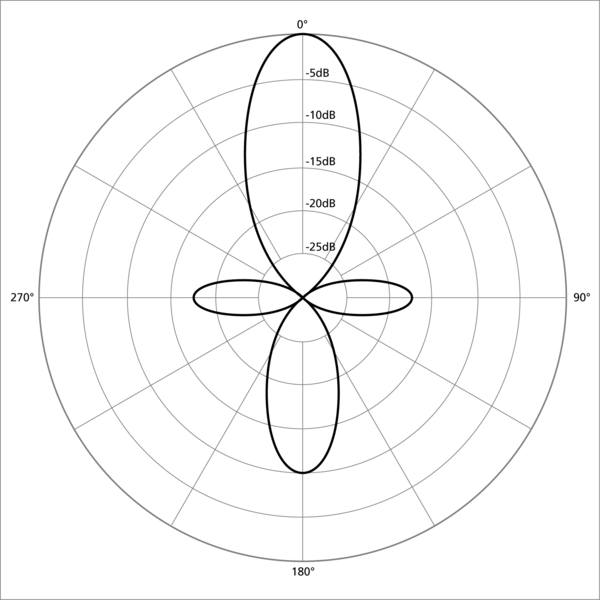
\includegraphics[width=0.4\textwidth]{abb6} 
	\caption[Keule]{Keule\footnotemark}
\end{figure}
\footnotetext{Quelle: https://www.delamar.de/mikrofon/richtcharakteristik-mikrofon-22647/}
\subsubsection{Acht}
Die sogenannte Achtcharakteristik nimmt den Schall von vorne und hinten auf, jedoch nur minimal von den Seiten. Diese Charakteristik hat die Verwendung bei der M/S-Stereofonie.\citep{kugel}\newline
Bei der M/S-Stereofonie, oder auch Mid/Side-Stereofonie, werden die Audiosignale mittig und von der Seite aufgenommen. In der Mitte befindet sich ein Mikrofon mit einer Nierencharakteristik, wohingegen die Seitensignale mit einer Achtcharakteristik aufgenommen werden. Die Seitensignale nehmen die Schallquellen aus unterschiedlichen Richtungen auf und sind so mit einem menschlichen Ohr zu vergleichen.\citep{ms}
\begin{figure}[H]
	\centering
	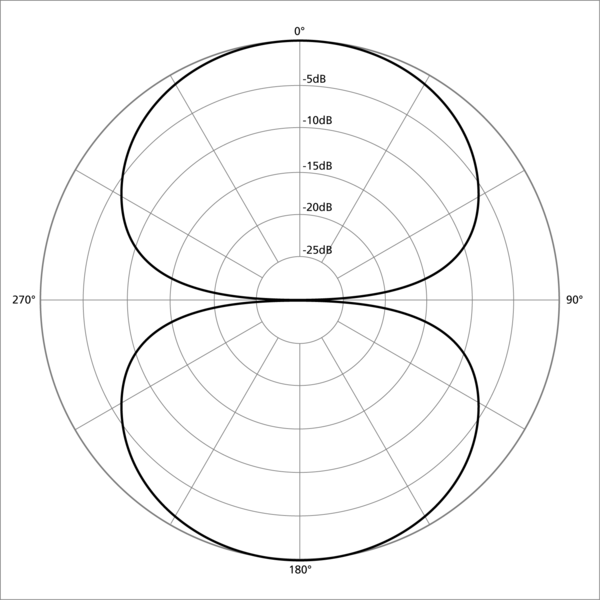
\includegraphics[width=0.4\textwidth]{abb7} 
	\caption[Acht]{Acht\footnotemark}
\end{figure}
\footnotetext{Quelle: https://www.delamar.de/mikrofon/richtcharakteristik-mikrofon-22647/}
\subsection{Kondensatormikrofon}
"Ein Kondensatormikrofon wandelt Schall in ein elektrisches Signal." (https://www.delamar.de/faq/kondensatormikrofon-34728/ [Zugriff: 17.03.2018])\newline
Bei einem Kondensatormikrofon treffen die Schallwellen zuerst auf die Membran, was eine leitende Folie ist, die mit Gold bedampft ist. Dies verbessert die  Leitfähigkeit des Mikrofons, was die Luftdruckschwankungen in mechanische Schwingungen umwandelt. Anschließend wird sie in elektrische Spannung umgewandelt und über die XLR-Buchse wieder ausgegeben.\citep{kondensator}
\begin{figure}[H]
	\centering
	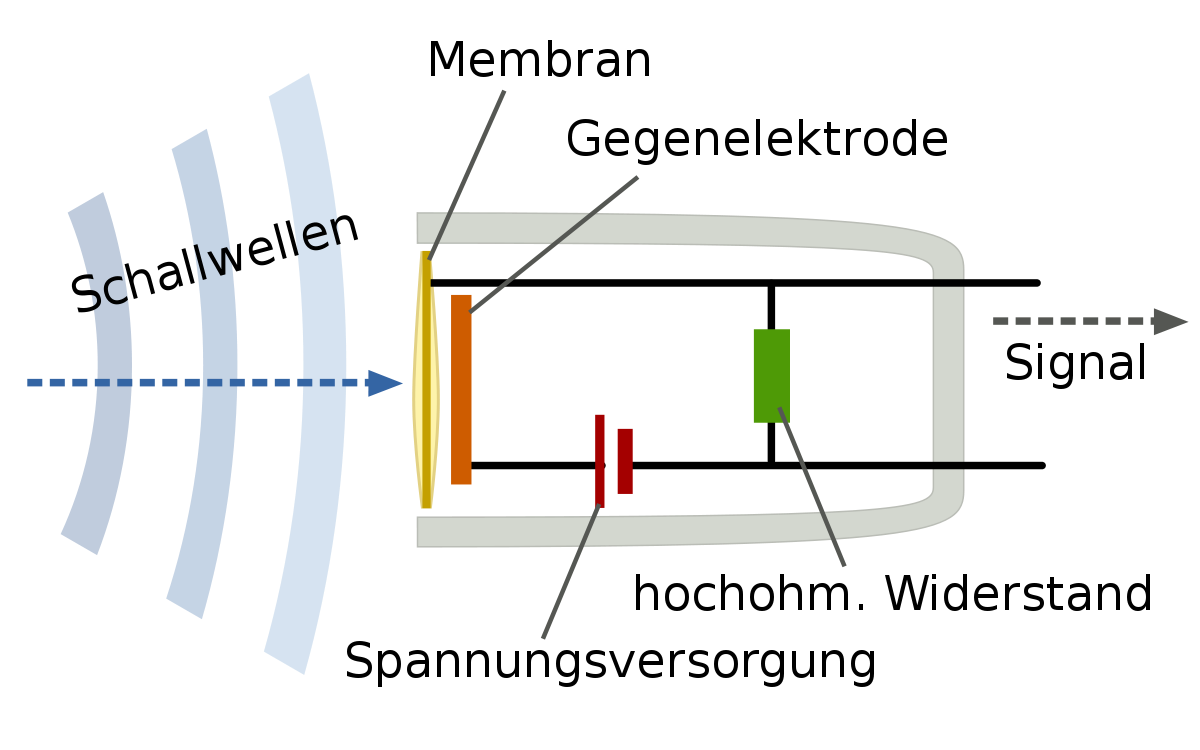
\includegraphics[width=0.6\textwidth]{abb8} 
	\caption[Kondensatormikrofon]{Kondensatormikrofon\footnotemark}
\end{figure}
\footnotetext{Quelle: https://de.wikipedia.org/wiki/Kondensatormikrofon\#/media/File:Kondensatormikrofon.svg}
\subsection{Dynamisches Mikrofon}
\begin{quote}
"Bei diesem Mikrofontyp wird das Signal durch elektromagnetische Induktion erzeugt. Kurz: Der Schall trifft auf die Membran des Mikrofons und regt sie zu mechanischen Schwingungen an, die durch eine mit der Membran verbundene Spule in elektrische Spannung umgewandelt werden. Und diese kommt dann aus der (XLR-)Buchse des Mikrofons." (https://www.delamar.de/faq/dynamisches-mikrofon-34718/ [Zugriff: 17.03.2018])
\end{quote} 
\begin{figure}[H]
	\centering
	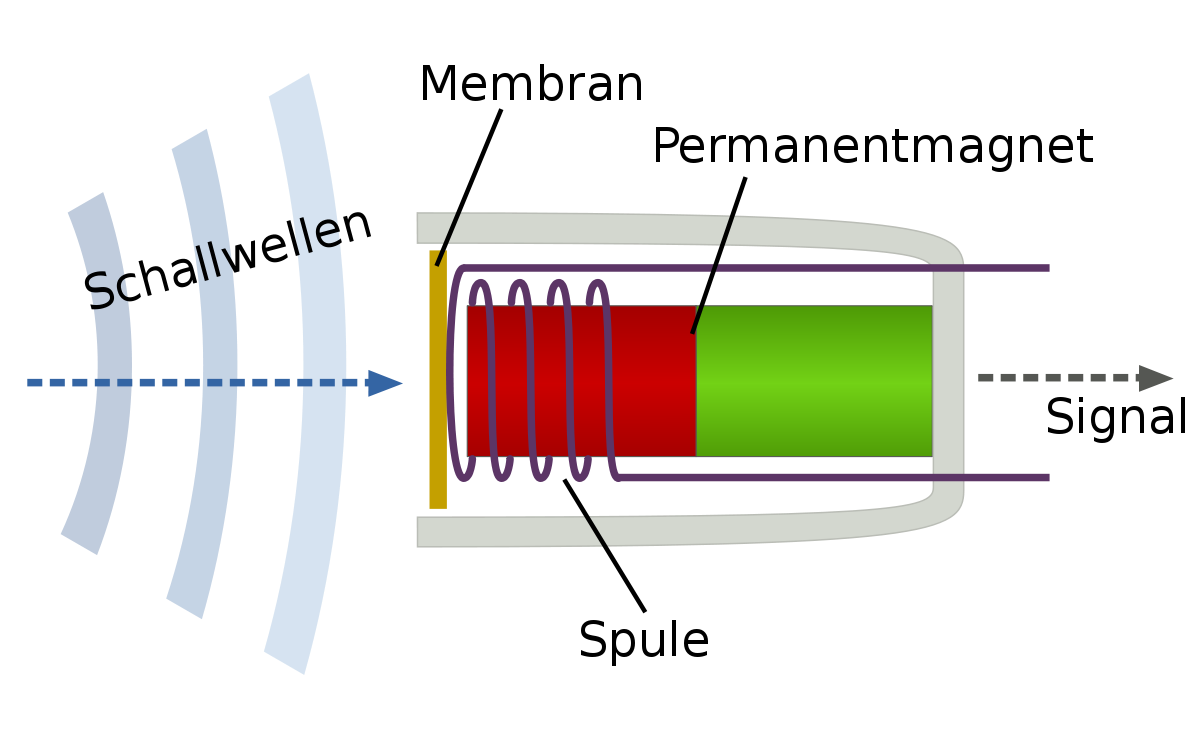
\includegraphics[width=0.6\textwidth]{abb9} 
	\caption[Dynamisches Mikrofon]{Dynamisches Mikrofon\footnotemark}
\end{figure}
\footnotetext{Quelle: https://de.wikipedia.org/wiki/Dynamisches\_Mikrofon\#/media/File:Tauchspulenmikrofon.svg}
\paragraph{Interview mit Abteilungsvorstand}
\leavevmode \\
Bei der Aufnahme des Videos mit dem Abteilungsvorstand Dr. Hager wurde das t-bone GZ 400 Grenzflächen-Mikrofon verwendet. Das Mikrofon arbeitet mit der Richtcharakteristik Halbniere. Das Mikrofon wurde in die Mitte des Tisches platziert, um die Stimmen der Interviewerin und des Abteilungsvorstandes einzufangen.\newline
Bei dem Video wurden bewusst keine Ansteckmikrofone verwendet, um nicht das typische Interview-Bild widerzuspiegeln, wo die Mikrofone an den Personen angesteckt werden und man diese dann auch im Video sieht.
\paragraph{Tag der offenen Tür}
\leavevmode \\
Bei dem Tag der offenen Tür Video wurde eine Angel für die Aufnahme der Interessenten verwendet. Hierfür wurde eine Keule beziehungsweise eine Superniere eingesetzt. Dies war deswegen notwendig, da am Tag der offenen Tür viele Hintergrundgeräusche vorhanden waren. Hätte man mit einer Kugelcharakteristik aufgenommen, würde man die Hintergrundgeräusche auch hören, im Gegensatz zu der Keule, welche hauptsächlich von vorne aufnimmt und Hintergrundgeräusche ausblendet.
\paragraph{Video mit einem Absolvent}
\leavevmode \\
Beim Quiz mit dem Absolventen und dem Schüler der zweiten Klasse wurde, wie beim ersten Interview, das Grenzflächen-Mikrofon verwendet.